\documentclass[11pt,a4paper]{article}
\usepackage[utf8]{inputenc}
\usepackage[T1]{fontenc}
\usepackage[spanish,es-tabla,es-nodecimaldot]{babel}
\usepackage{lmodern}
\usepackage[margin=2.5cm]{geometry}
\usepackage{booktabs,graphicx,xcolor,array,float,caption,amsmath,amssymb,enumitem,longtable,ragged2e}
\usepackage[hidelinks]{hyperref}
\usepackage{microtype}
\graphicspath{{../assets/}}
\setlength{\parindent}{0pt}
\setlength{\parskip}{0.55em}
\renewcommand{\arraystretch}{1.15}
\captionsetup{font=small,labelfont=bf}
\setlist{itemsep=0.15em,topsep=0.3em}
\newcommand{\codigo}[1]{\texttt{\detokenize{#1}}}
\newcommand{\pend}[1]{\textcolor{red!60!black}{[#1]}}

\title{\textbf{Dark Forest: necesitar a los otros, temer a los otros}\\[0.4em]
\large Aprendizaje por refuerzo multiagente en un juego estoc\'astico parcialmente observable\\[0.3em]
\normalsize Proyecto final de CC3104, Aprendizaje por Refuerzo}
\author{Ricardo Chuy (221007), Sergio Orellana (221122), Rodrigo Mansilla (22611),\\ M\'onica Salvatierra (22249) y Bianca Calder\'on (22272)\\ Secci\'on 10}
\date{Noviembre de 2026}

\begin{document}
\maketitle

\begin{abstract}
\noindent Varias civilizaciones simuladas crecen en un toro bidimensional. Una anomal\'ia c\'iclica las amenaza y solo puede predecirse combinando mediciones de al menos dos de ellas, pero comunicarse revela la posici\'on y otra civilizaci\'on puede atacar. Se construy\'o el entorno en JAX, un conjunto de estrategias fijas de referencia, un entrenamiento IPPO con GRU y una demo web que reproduce los episodios. Con estrategias fijas, cooperar aporta entre $+0.2$ y $+3.9$ de retorno seg\'un la letalidad y el tama\~no de la zona (con letalidad cero no aporta nada). Con redes entrenadas, el cuello de botella fue el entrenamiento: desde cero las redes colapsan a $+2.84$, cerca de ignorar a las dem\'as ($+2.97$), y con imitaci\'on previa de una estrategia cooperativa llegan a $+4.37$, sin alcanzar a esa estrategia ($+5.99$). De las cinco hip\'otesis, H1 se confirma, H2 se apoya en parte (la dependencia del canal crece con la velocidad de la se\~nal a letalidad baja) y H3, H4 y H5 quedan como preguntas abiertas para este entorno. El documento separa lo medido de lo interpretado e indica el alcance de cada cifra.
\end{abstract}

\tableofcontents
\newpage

%% ------------------------------------------------------------------
\section{Descripci\'on del problema}

La hip\'otesis del bosque oscuro de Liu Cixin \cite{liu2015} sostiene que, si la intenci\'on de otra civilizaci\'on no puede verificarse, esconderse o atacar primero puede ser lo racional. El proyecto toma como punto de partida el escenario C de \textit{Rogue Agents}: varios agentes reciben un desaf\'io que ninguno resuelve solo, perciben el universo de forma parcial e individual, compiten por recursos y pueden eliminarse entre s\'i. Se busca saber si emergen coaliciones, conflicto, negociaci\'on o colapso.

El problema de dise\~no es que, en el bosque oscuro cl\'asico, el contacto solo trae riesgo. Si el entorno se construye as\'i, esconderse o atacar domina de forma trivial y no emerge nada: el resultado ya est\'a en las reglas. El contrapeso que propone el proyecto es un \emph{desaf\'io compartido}: una anomal\'ia peri\'odica cuyos par\'ametros ocultos $\theta$ solo se identifican combinando al menos dos proyecciones ruidosas. Comunicarse vale algo, pero comunicarse revela la posici\'on. El dilema central es:

\begin{quote}
\emph{Necesito a los otros para sobrevivir, pero los otros pueden destruirme si me encuentran.}
\end{quote}

\textbf{Pregunta de investigaci\'on.} \textquestiondown Cu\'anto debe valer la cooperaci\'on para vencer al miedo, y c\'omo cambia ese umbral con el retraso de las se\~nales, la letalidad de los ataques y la posibilidad de enviar se\~nales costosas?

\textbf{Resultado esperado.} Un diagrama de fases que muestre en qu\'e condiciones aparece cada r\'egimen: cooperaci\'on, silencio mutuo, ataque preventivo, coaliciones o colapso.

\textbf{Criterio de no imposici\'on.} La recompensa de cada civilizaci\'on es solo el crecimiento logar\'itmico de sus recursos,
\begin{equation}
R_{i,t}=\log(1+r_{i,t+1})-\log(1+r_{i,t}),
\end{equation}
sin t\'erminos por ocultarse, atacar o cooperar. Cualquier estrategia que aparezca debe ser instrumental. Este criterio es lo que hace que la pregunta sea cient\'ifica y no un resultado de dise\~no.

%% ------------------------------------------------------------------
\section{An\'alisis}

\subsection{Formalizaci\'on}

El juego es un juego estoc\'astico parcialmente observable (POSG) \cite{hansen2004}, $\langle N, S, \{A_i\}, \{O_i\}, T, \{R_i\}, \gamma\rangle$, con $N\in\{2,4,6,8\}$ civilizaciones. Cada una ve solo su observaci\'on $o_i$ y no conoce $N$ ni las posiciones de las dem\'as. Las posiciones son fijas y viven en un toro $[0,1)^2$, es decir, un cuadrado cuyos lados opuestos se identifican; las distancias se miden por el camino m\'as corto a trav\'es de los bordes. Hay siete acciones: crecer, ocultarse, observar, transmitir un s\'imbolo, compartir la \'ultima medici\'on, atacar y refugiarse. Las se\~nales se expanden como anillos de radio $c\,(t-t_{\text{emisi\'on}})$ y los proyectiles viajan a una velocidad menor o igual que $c$. Descubrir a otra civilizaci\'on es que su cono de luz alcance a la propia.

\subsection{Lo que el an\'alisis inicial mostr\'o}

Antes de entrenar, se midieron estrategias escritas a mano para saber si las reglas dejaban algo que aprender (cap\'itulo~\ref{sec:resultados}). Tres hallazgos cambiaron el dise\~no:

\begin{enumerate}
\item \textbf{Con periodo fijo de la anomal\'ia, cooperar no compensa.} Una civilizaci\'on sola ya despejaba la fase con su propia medici\'on. Se sortea ahora el periodo por episodio (par\'ametro \codigo{anomaly.period_spread}); es un arreglo de fidelidad, porque la propuesta ya define el periodo como par\'ametro oculto.
\item \textbf{Con las reglas originales, el ataque no es una decisi\'on interesante.} Con recompensa logar\'itmica y crecimiento exponencial, sobrevivir 200 pasos creciendo vale cerca de $9$ y morir cuesta menos de $1$. Renunciar a crecer solo conviene si la probabilidad de sobrevivir creciendo es menor que cerca de 7\,\%.
\item \textbf{Cooperar no costaba exposici\'on.} Crecer ya emit\'ia en alta, as\'i que compartir no revelaba nada nuevo. El par\'ametro \codigo{env.detection_growth} permite que crecer sea silencioso y que compartir sea el \'unico acto visible.
\end{enumerate}

Una consecuencia de estos hallazgos es que la hip\'otesis H1 se reformul\'o despu\'es de ver datos (secci\'on~\ref{sec:hipotesis}); el cambio se declara como tal.

\subsection{Hip\'otesis}
\label{sec:hipotesis}

\begin{table}[H]
\centering\small
\begin{tabular}{@{}l p{9.2cm} p{3.2cm}@{}}
\toprule
ID & Hip\'otesis & Prueba \\
\midrule
H1 & Con $\lambda=0$ la cooperaci\'on no tiene valor: anular el canal no cambia retorno ni supervivencia. & Ablaci\'on del canal \\
H2 & Existe un $\lambda^*$ desde el cual emerge la comunicaci\'on, y crece con el retraso y con $p_{\text{kill}}$. & Barrido $\lambda\times c$ \\
H3 & Se\~nales caras de falsificar reducen $\lambda^*$. & Barrido con y sin se\~nales costosas \\
H4 & Con $N\ge 6$ y detecci\'on local aparecen grupos que comparten entre s\'i y callan ante los dem\'as. & Grafo de mensajes y comunidades \\
H5 & Cerca de $\lambda^*$ unas seeds convergen a cooperaci\'on y otras a silencio. & Distribuci\'on por seed \\
\bottomrule
\end{tabular}
\caption{Hip\'otesis falsables del proyecto. $\lambda$ es la letalidad de la anomal\'ia y $c$ la velocidad de las se\~nales.}
\end{table}

La redacci\'on original de H1 dec\'ia que con $\lambda=0$ el silencio o el ataque preventivo dominan. Se midi\'o que crecer es la mejor respuesta a todas las estrategias probadas, as\'i que H1 pas\'o a ser la prueba de cordura de que el canal no filtra informaci\'on. La pregunta original se conserva como exploratoria.

\subsection{Criterios para distinguir emergencia genuina}

Se exigi\'o no imposici\'on, necesidad funcional (anular el canal y barajar los mensajes), modelo nulo (agentes aleatorios y arquetipos), robustez (cinco seeds o m\'as) y dependencia de condiciones (barrido de par\'ametros).

%% ------------------------------------------------------------------
\section{Propuesta de soluci\'on}

La soluci\'on tiene cuatro piezas que se apoyan una en otra:

\begin{enumerate}
\item \textbf{Un simulador r\'apido y reproducible} escrito en JAX, para entrenar miles de episodios en paralelo.
\item \textbf{Estrategias fijas de referencia} (ignorar, solo, cooperadora, rec\'iproca, prudente, mentirosa, atacante) que act\'uan como modelo nulo, techo y rivales de evaluaci\'on.
\item \textbf{Agentes entrenados} con IPPO sobre una red recurrente (GRU) con par\'ametros compartidos, autojuego con poblaci\'on y, cuando el entrenamiento desde cero no converge, imitaci\'on previa de una estrategia cooperativa.
\item \textbf{Una demo web} que simula un episodio con las pol\'iticas elegidas y lo muestra, de modo que el comportamiento pueda inspeccionarse y no solo medirse.
\end{enumerate}

El orden importa. Las estrategias fijas se midieron primero para decidir qu\'e reglas dejaban algo que aprender; los agentes entrenados se compararon siempre contra esas referencias; y la demo se construy\'o al final, sobre los mismos episodios que produce el simulador, sin cambiar los datos.

%% ------------------------------------------------------------------
\section{Descripci\'on de la soluci\'on}

\subsection{Arquitectura del repositorio}

\begin{table}[H]
\centering\small
\begin{tabular}{@{}l p{10cm}@{}}
\toprule
M\'odulo & Responsabilidad \\
\midrule
\codigo{darkforest/} & Configuraci\'on, tipos, entorno puro (\codigo{reset}, \codigo{step}), anomal\'ia, pol\'iticas, arquetipos y red actor-cr\'itico GRU \\
\codigo{train/} & IPPO, poblaci\'on de autojuego, barrido, imitaci\'on, diagn\'osticos con pol\'iticas fijas \\
\codigo{analysis/} & M\'etricas, replicador, diagrama de fases, coaliciones, barrido entrenado \\
\codigo{viz/} & Animaci\'on y exportaci\'on de episodios a JSON \\
\codigo{demo/} & Servidor local y p\'agina web con capa narrativa \\
\bottomrule
\end{tabular}
\caption{M\'odulos y sus responsabilidades. Las dependencias van en un solo sentido: \codigo{train}, \codigo{analysis} y \codigo{viz} importan a \codigo{darkforest}, nunca al rev\'es.}
\end{table}

\subsection{Entorno}

El entorno es una funci\'on pura de estado y acciones, compatible con \codigo{jit} y \codigo{vmap}. El estado contiene posiciones, recursos, vida, nivel de emisi\'on, par\'ametros ocultos $\theta$ de la anomal\'ia y las colas de se\~nales y proyectiles. Cada estallido de la anomal\'ia mata, con probabilidad $\lambda$, a toda civilizaci\'on dentro de la zona que no est\'e refugiada. Refugiarse siempre cuesta, as\'i que no puede hacerse en todos los turnos: hay que predecir cu\'ando.

Se a\~nadieron mec\'anicas como par\'ametros, apagadas o neutras por defecto, para no elegir reglas por su efecto: \codigo{anomaly.period_spread}, \codigo{env.detection_growth}, \codigo{env.detection_transmit}, \codigo{env.loot}, \codigo{env.projectiles_cancel_on_death}, y, para H3, \codigo{env.deception}, \codigo{env.costly_signals} y \codigo{env.cost_verify}.

\subsection{Agentes y entrenamiento}

La red es un actor-cr\'itico con una GRU de 128 unidades, compartida entre civilizaciones y diferenciada por un identificador. Se entrena con PPO independiente por agente (IPPO). En la configuraci\'on base: 1024 entornos en paralelo, rollouts de 64 pasos, tasa de aprendizaje $3\times10^{-4}$, $\gamma=0.99$, GAE con $\lambda_{\text{GAE}}=0.95$ y recorte $0.2$. El entrenamiento usa una poblaci\'on: con probabilidad $\rho$ cada civilizaci\'on adopta una pol\'itica de la poblaci\'on (versiones pasadas congeladas y estrategias fijas) y no la pol\'itica en entrenamiento.

Como las redes entrenadas desde cero no convergieron, se a\~nadi\'o un procedimiento en tres etapas: (1) clonar a la estrategia cooperativa \codigo{coop_real} mediante entrop\'ia cruzada sobre sus acciones y regresi\'on de su valor; (2) corregir la desviaci\'on con DAgger \cite{ross2011}; (3) afinar con RL en poblaci\'on mixta. Ninguna de las tres etapas toca el entorno ni la recompensa.

\subsection{Evaluaci\'on}

Cada red se eval\'ua de dos maneras: por \emph{muestreo} (la acci\'on se saca de la distribuci\'on de la pol\'itica) y en modo \emph{greedy} (la acci\'on de mayor probabilidad). Se informan las dos, porque con muestreo una probabilidad cercana a 1\,\% de atacar produce casi un disparo por episodio y oculta lo que la red aprendi\'o. Las referencias (ignorar, solo, pareja \codigo{coop_real}, or\'aculo) se miden en el mismo mundo. Una matriz de cruce enfrenta redes y estrategias entre s\'i.

\subsection{Demo web}

La demo sirve la p\'agina y dos rutas (\codigo{/api/opciones} y \codigo{/api/simular}). Corre el simulador con el mundo y las pol\'iticas elegidos y devuelve el episodio exportado a JSON. Hay un modo cient\'ifico (discos, anillos, leyenda y tabla, de referencia para comparar escenas) y un modo narrativo (sistemas estelares con planeta y astronauta, escala de Kardashev ilustrativa, flotas, ficha de civilizaci\'on y bit\'acora). La regla es que la decoraci\'on nunca afirme algo que los datos no digan: el aspecto del planeta, el nombre del sistema y la etapa de Kardashev son decorativos; posiciones, recursos, acciones, se\~nales, proyectiles, estallidos y muertes son los datos del episodio. Un cat\'alogo de 12 escenarios permite presentar sin servidor.

%% ------------------------------------------------------------------
\section{Herramientas aplicadas}

Del curso se usan: el marco de RL, la observaci\'on parcial (POMDP) y los MDP con las ecuaciones de Bellman (S1, S3); gradiente de pol\'itica, actor-cr\'itico, funci\'on de ventaja, GAE, PPO con recorte y t\'ermino de entrop\'ia (S8); DQN y \emph{experience replay} (S12); y aprendizaje multiagente, con los aprendices independientes (IPPO), el entrenamiento centralizado y ejecuci\'on descentralizada, MAPPO y la comunicaci\'on aprendida (DIAL, RIAL, CommNet) (S15). Los m\'etodos tabulares (bandidos, programaci\'on din\'amica, Monte Carlo, TD, Dyna) sirven como fundamento. Lo que no forma parte de las sesiones se elabora a continuaci\'on: JAX, la GRU, el autojuego ficticio, la clonaci\'on de comportamiento y DAgger, la din\'amica del replicador, las se\~nales costosas, y las herramientas de c\'omputo y visualizaci\'on. Las herramientas siguientes se elaboran con m\'as detalle.

\subsection{JAX: \texttt{jit}, \texttt{vmap} y n\'umeros aleatorios expl\'icitos}

JAX \cite{bradbury2018} es una biblioteca de c\'omputo num\'erico que compila funciones de Python a c\'odigo para CPU o GPU mediante XLA. Tres ideas bastan para entender por qu\'e se eligi\'o:

\begin{itemize}
\item \codigo{jax.jit} compila una funci\'on una vez y la reutiliza. Por eso cada mundo nuevo obliga a recompilar el simulador (30 a 60 segundos en CPU) y los episodios siguientes del mismo mundo son r\'apidos.
\item \codigo{jax.vmap} convierte una funci\'on de un episodio en una de un lote, sin escribir bucles. Es lo que permite simular 1024 entornos a la vez.
\item La aleatoriedad es expl\'icita: no hay estado global. Cada \codigo{PRNGKey} se pasa y se divide con \codigo{split}. Esto hace que un episodio sea reproducible dada su semilla, que es una regla del proyecto.
\end{itemize}

La contrapartida es que el entorno debe ser una funci\'on pura con formas est\'aticas, sin efectos secundarios; por eso se prohibi\'o \codigo{print} y estado global en \codigo{darkforest/}. Un entorno en JAX tambi\'en hace posible el trabajo en GPU: los entrenamientos finales corrieron en Kaggle con GPU T4 (dos en paralelo). Trabajos como JaxMARL \cite{rutherford2023} usan el mismo enfoque para entornos multiagente.

\subsection{IPPO, parámetros compartidos y GRU}

IPPO \cite{dewitt2020} entrena a cada agente con PPO \cite{schulman2017} tratando a los dem\'as como parte del entorno; MAPPO \cite{yu2022} a\~nade un cr\'itico con informaci\'on global. Se eligi\'o IPPO porque cada civilizaci\'on solo ve su observaci\'on y porque, con par\'ametros compartidos, una sola red sirve para cualquier $N$ (se evalu\'o con $N$ distinto del de entrenamiento sin reentrenar). La GRU \cite{cho2014} lleva una memoria que resume lo visto, necesaria porque la informaci\'on es parcial y las se\~nales llegan con retraso.

El autojuego ficticio \cite{heinrich2016} entrena contra versiones pasadas de la propia red para no quedar atrapado en un solo equilibrio. En este proyecto la poblaci\'on tambi\'en incluye estrategias fijas (cooperadora, rec\'iproca, atacante, solo, ignorar).

\subsection{Imitaci\'on y DAgger}

La clonaci\'on de comportamiento entrena una red para reproducir las acciones de un experto con entrop\'ia cruzada. Su problema es que la red, al equivocarse, visita estados que el experto nunca mostr\'o y all\'i no sabe qu\'e hacer. DAgger \cite{ross2011} lo corrige: la red juega, el experto etiqueta los estados que la red visita, y se vuelve a entrenar con ese conjunto ampliado. Aqu\'i el experto es la estrategia fija \codigo{coop_real} y se usaron 4 rondas. Se a\~nadieron pesos por rareza, porque lo que importa son pocos pasos cr\'iticos (refugiarse en el estallido) entre muchos triviales.

\subsection{Din\'amica del replicador y masas cr\'iticas}

La din\'amica del replicador \cite{taylor1978} describe c\'omo cambia la fracci\'on de cada estrategia en una poblaci\'on seg\'un su pago relativo. Se midi\'o una matriz de pagos entre estrategias en el mismo simulador y se estudi\'o hacia d\'onde converge una poblaci\'on. Como la cuenca de atracci\'on depende de la mezcla inicial elegida, se report\'o tambi\'en la \emph{masa cr\'itica}: la fracci\'on de una estrategia a partir de la cual vence a otra en el juego de esas dos. Con eso se construy\'o el diagrama de reg\'imenes $\lambda\times c$.

\subsection{Cheap talk y se\~nales costosas}

H3 viene de la teor\'ia de se\~nales. Un mensaje que cuesta lo mismo decir verdad que mentir no compromete a nadie \cite{crawford1982}; una se\~nal cuyo costo es distinto seg\'un el tipo del emisor puede separar tipos \cite{spence1973}. Se implement\'o as\'i: con \codigo{costly_signals} el compartir verdadero cuesta m\'as (0.06 contra 0.02) y lleva una etiqueta de verificado que la mentira no puede emitir. La comunicaci\'on emergente entre agentes de aprendizaje por refuerzo tiene su propia literatura \cite{foerster2016,lazaridou2020}.

\subsection{Entorno de c\'omputo: uv, Kaggle y killswitch}

Las dependencias se fijan con \codigo{uv} (\codigo{uv.lock}); cualquier comando va con \codigo{uv run}. Los entrenamientos largos corrieron en Kaggle (GPU T4), con un \emph{killswitch}: un interruptor dentro del kernel que lo detiene si supera las cinco horas, para no consumir el presupuesto en una corrida atascada.

\subsection{Visualizaci\'on: three.js, PyVista y un sistema de dise\~no}

La vista 3D de la web usa three.js; una vista fuera de l\'inea usa PyVista \cite{sullivan2019}. El estilo visual sale de un sistema de dise\~no propio (dos temas, noche y carta) con tokens y componentes, de modo que la interfaz no lleve colores sueltos. La capa narrativa se escribi\'o como m\'odulos independientes (astronauta, planetas, escala de Kardashev \cite{kardashev1964}, efectos, bit\'acora, ficha de civilizaci\'on) con un contrato com\'un y pruebas en Node. La escala de Kardashev es ilustrativa: los recursos son adimensionales y la etapa no mide energ\'ia.

Una decisi\'on f\'isica de la vista 3D: el mapa es un toro, as\'i que las distancias y las copias al otro lado del borde se dibujan como son. El tama\~no de cada sistema se reduce para no solaparse con el vecino m\'as cercano, medido por el camino m\'as corto a trav\'es de los bordes.

\subsection{IA generativa: prompts y evoluci\'on de la idea}
\label{sec:prompts}

La herramienta fue Claude Code (Anthropic), un agente de c\'odigo en la terminal, con modelos de la familia Claude \cite{anthropicclaudecode}. Tambi\'en se us\'o un paquete de \emph{skills} de escritura cient\'ifica en formato Agent Skills \cite{agentskills} para estructurar este documento. Los prompts se reproducen abreviados y en el orden en que se dieron; no se corrigi\'o su redacci\'on.

\begin{longtable}{@{}p{2.0cm} p{7.4cm} p{5.6cm}@{}}
\caption{Prompts principales y qu\'e produjeron.}\label{tab:prompts}\\
\toprule
Fecha & Prompt (abreviado) & Efecto \\
\midrule
\endfirsthead
\toprule
Fecha & Prompt (abreviado) & Efecto \\
\midrule
\endhead
23 oct. & \textit{``arma un esqueleto para el proyecto''}, con la propuesta completa pegada (13\,000 caracteres) & Esqueleto del repositorio: configuraci\'on, entorno, pruebas \\
23 oct. & \textit{``usemos uv''} & Dependencias fijadas con \codigo{uv.lock} \\
25 oct. & \textit{``se par\'o por l\'imites de uso, retoma donde se qued\'o y si termin\'o alg\'un notebook de kaggle, verif\'icalo''} & Se retom\'o el trabajo y se verific\'o un notebook \\
26 oct. & \textit{``d\'ejame un listado de tareas para un grupo de 5 personas, yo quiero solo supervisar y hacer ajustes''} & \codigo{docs/TODO.md} y \codigo{docs/TAREAS.md} \\
7 nov. & \textit{``mira qu\'e hace falta: lineamiento, objetivo principal, idea principal, propuesta principal [\ldots] entiendo que no converge [\ldots] \textquestiondown d\'onde no estamos viendo? [\ldots] podemos salirnos un poquito de la caja''} & Informe de estado y de lo que faltaba; plan de diagn\'osticos y extensiones \\
8 nov. & \textit{``\textquestiondown conviene probar Prime Intellect?''}, precios y \textit{``deja un killswitch si tarda m\'as de 5 hrs''} & Se decidi\'o usar Kaggle como presupuesto de c\'omputo; se a\~nadi\'o el interruptor \\
9 nov. & \textit{``dame next steps para despu\'es de las pruebas, qu\'e extensiones consideradas y no consideradas podemos hacer''} & Lista de extensiones (imitaci\'on, explotadores, $N$ grande, H3) \\
9 nov. & \textit{``hacer un barrido grande que tome estas variables, ya si no funcionan se reportan y sirven como resultado''}, con lista de hip\'otesis & Barrido $\lambda\times c$ con redes, juego emp\'irico y explotadores \\
9 nov. & \textit{``para una visualizaci\'on, \textquestiondown se va a poder ajustar pol\'iticas e inferencia sobre lo ya entrenado? [\ldots] simular diferentes mundos''} & Servidor de simulaci\'on en vivo con redes y estrategias \\
9 nov. & \textit{``Mejora la ui con un panel en design [\ldots] visualizaci\'on 3D con pyvista o vispy''} & Sistema de dise\~no y visor PyVista \\
9 nov. & Error pegado: \textit{``mul got incompatible shapes for broadcasting: (1, 6), (1, 2)''} & Correcci\'on de la simulaci\'on para $N>2$ \\
9 nov. & \textit{``\textquestiondown hay manera de no entrenar y estimar/aproximaci\'on?''} & Evaluar redes de 2 y 6 civilizaciones con otro $N$ sin reentrenar \\
9 nov. & \textit{``no se entiende c\'omo crecen ni qu\'e son galaxias o planetas [\ldots] skin por planeta [\ldots] escala de Kardashev [\ldots] animar ataques con probes y flotas''} & Capa narrativa: galaxia, planetas, Kardashev, flotas \\
9 nov. & \textit{``hace todo usa agentes. Quiero que tengan skins de astronauta''} & Seis m\'odulos escritos por agentes en paralelo con un contrato com\'un \\
9 nov. & \textit{``no me termina de convencer el toro, no parece una galaxia; la animaci\'on 2D y 3D tambi\'en se ven mal''} & Fondo de galaxia, nube de anomal\'ia, tiempo fraccionario \\
10 nov. & \textit{``quiero algo as\'i''} con la ruta de un proyecto propio de sistema solar & Vista 3D estilo sistema solar: estrellas, \'orbitas, salto warp \\
10 nov. & \textit{``ajusta c\'omo se muestran $n>2$ galaxias, respetemos la f\'isica''} & Escala fiel por distancia m\'inima y copias al otro lado del borde \\
\bottomrule
\end{longtable}

\textbf{Valoraci\'on de las respuestas.} Los prompts que dieron buen resultado fueron los que pidieron un entregable concreto y verificable: el esqueleto con la propuesta completa, el listado de tareas, el barrido con la lista de hip\'otesis y los cambios de la demo con un criterio visual claro. Los que no respondieron bien fueron los vagos o los que dejaron decidir a la herramienta: el primer intento de vista 3D ``tipo toro'' no se le\'ia como galaxia, el conteo de mensajes de coaliciones contaba cualquier se\~nal, y varios errores (formas incompatibles para $N>2$, hojas de estilo con tipo de contenido incorrecto, un cat\'alogo con una sola pol\'itica para seis civilizaciones) aparecieron solo al ejecutar. La causa com\'un fue que la herramienta generaba c\'odigo plausible sin probarlo en el caso general; por eso cada cifra se contrast\'o con pruebas y con ejecuciones reales y no con la afirmaci\'on de la herramienta. La IA aceler\'o la escritura del entorno, las pruebas y la demo; las decisiones de dise\~no, la reformulaci\'on de H1 y la interpretaci\'on de resultados fueron del equipo.

\textbf{Evoluci\'on de la idea.} El trabajo pas\'o por cuatro fases.

\begin{enumerate}
\item \emph{Construir seg\'un la propuesta.} Se implement\'o el entorno y el entrenamiento tal como estaban especificados. El entrenamiento no converg\'ia a ``solo crecer'' ni usaba el canal.
\item \emph{Diagnosticar antes de seguir entrenando.} En lugar de entrenar m\'as, se midieron estrategias fijas. Eso mostr\'o que parte del problema estaba en las reglas (cooperar no costaba nada, el periodo fijo era identificable) y llev\'o a reformular H1 y a a\~nadir par\'ametros.
\item \emph{Atacar la optimizaci\'on.} Tres cambios (minibatches, escala de recompensa, entrop\'ia decreciente) sacaron a las redes del peor colapso, y la imitaci\'on con DAgger fue la \'unica forma encontrada de salir del colapso con refugio caro.
\item \emph{Hacer visible el comportamiento.} La demo y su capa narrativa, iterada contra el criterio del autor: se retiraron elementos que confund\'ian (pilares de recursos) y se reemplazaron por tama\~no del disco y r\'otulos.
\end{enumerate}

\textbf{Qu\'e fall\'o y c\'omo se corrigi\'o.} Un an\'alisis de coaliciones contaba cualquier se\~nal recibida como mensaje; se separ\'o el conteo de mensajes expl\'icitos y se document\'o que la conclusi\'on depende del umbral. Una publicaci\'on de la demo como p\'agina alojada se descart\'o porque el autor prefiri\'o la demo local con simulaci\'on en vivo. La vista 3D con forma de toro se reemplaz\'o porque no se le\'ia como galaxia. El servidor entregaba las hojas de estilo con un tipo de contenido incorrecto y la p\'agina sal\'ia sin estilo. Un escenario del cat\'alogo con una sola pol\'itica para seis civilizaciones fall\'o hasta duplicar la pol\'itica.

\subsection{Entendimiento de la soluci\'on}

El simulador es una funci\'on pura que avanza el estado un turno. El valor de comunicarse no est\'a en la recompensa sino en la f\'isica: la anomal\'ia solo se puede predecir juntando dos mediciones, y refugiarse a ciegas cuesta. Las redes aprenden a refugiarse al ritmo de los estallidos usando una observaci\'on p\'ublica (los turnos desde el \'ultimo estallido), y con refugio barato eso basta, as\'i que no necesitan comunicarse. Con refugio caro comunicarse rinde, pero el entrenamiento desde cero no encuentra el protocolo; la imitaci\'on s\'i lo aproxima.

Cinco decisiones sostienen el dise\~no. (1) La recompensa es solo el cambio del logaritmo de los recursos, as\'i que no impone cooperar ni atacar. (2) Se midieron estrategias fijas antes de entrenar, y eso cambi\'o las reglas del entorno. (3) H1 se reformul\'o despu\'es de ver datos y as\'i se reporta. (4) El cuello de botella de las redes es el descubrimiento del protocolo, y la imitaci\'on lo reduce. (5) Los resultados negativos de H3, H4 y H5 se reportan igual que los positivos.

Dos preguntas quedan abiertas como l\'imites de la explicaci\'on: por qu\'e la red clonada llega a entre 61\,\% y 94\,\% de la estrategia que imita y no m\'as, y de d\'onde sale exactamente la ganancia de las redes afinadas sobre la heur\'istica \codigo{solo}.

%% ------------------------------------------------------------------
\section{Resultados (m\'etricas)}
\label{sec:resultados}

\subsection{C\'omo se mide}

El retorno es la suma de la recompensa de cada civilizaci\'on en 200 pasos. Las cifras con $\pm$ son errores est\'andar entre seeds. Los entrenados usan 5 seeds por configuraci\'on salvo que se indique; las estrategias fijas, 3 a 5 seeds y 100 a 400 episodios seg\'un la tabla. Cada tabla dice con qu\'e muestra se calcul\'o.

\subsection{Estrategias fijas}

\textbf{El aporte de cooperar depende del periodo de la anomal\'ia y de la letalidad.} Con periodo fijo, compartir cuesta m\'as de lo que informa (aporte real entre $-0.20$ y $-0.24$). Con periodo aleatorio el aporte real es positivo y crece con $\lambda$ hasta 0.5.

\begin{table}[H]
\centering\small
\begin{tabular}{@{}llrrr@{}}
\toprule
Mundo & $\lambda$ & \codigo{solo} & \codigo{coop_real} & Aporte real \\
\midrule
periodo fijo & 0.5 & 8.233 & 8.013 & $-0.219\pm0.025$ \\
periodo aleatorio & 0.25 & 7.764 & 7.946 & $+0.183\pm0.060$ \\
periodo aleatorio & 0.5 & 7.272 & 7.765 & $+0.493\pm0.081$ \\
periodo aleatorio & 1.0 & 6.954 & 7.456 & $+0.502\pm0.063$ \\
\bottomrule
\end{tabular}
\caption{Retorno medio por civilizaci\'on con dos civilizaciones, 400 episodios por seed y 5 seeds. El aporte es \codigo{coop_real} menos \codigo{solo}. El techo del or\'aculo es 8.96.}
\end{table}

\textbf{Ablaci\'on del canal (H1 con estrategias fijas).} Con $\lambda=0$ apagar el canal cambia el retorno de \codigo{coop_real} en menos de $0.05$ y con signo distinto seg\'un el radio de la zona; con $\lambda>0$ el canal importa y su aporte crece con $\lambda$ y con el radio. Las estrategias \codigo{ignorar} y \codigo{solo} rinden lo mismo con y sin canal en las ocho celdas, seed por seed: no hay fuga de informaci\'on.

\begin{table}[H]
\centering\small
\begin{tabular}{@{}rrrrr@{}}
\toprule
$\lambda$ & radio & con canal & sin canal & aporte del canal \\
\midrule
0 & 0.25 & $+8.383$ & $+8.337$ & $-0.682\pm0.005$ \\
0 & 0.45 & $+8.215$ & $+8.258$ & $-0.850\pm0.004$ \\
0.5 & 0.25 & $+7.917$ & $+6.840$ & $+0.677\pm0.128$ \\
0.5 & 0.45 & $+7.254$ & $+3.643$ & $+3.543\pm0.153$ \\
1 & 0.25 & $+7.778$ & $+6.508$ & $+0.709\pm0.106$ \\
1 & 0.45 & $+6.681$ & $+2.503$ & $+3.900\pm0.151$ \\
\bottomrule
\end{tabular}
\caption{Ablaci\'on del canal para \codigo{coop_real} (seis de las ocho celdas medidas; el aporte es respecto de la mejor entre ignorar y solo). Dos civilizaciones, 5 seeds, 200 episodios.}
\end{table}

Barajar los mensajes (conservar emisor y llegada pero cambiar la medici\'on por la de otro episodio) quita casi todo lo que quita apagar el canal: lo que vale es que el mensaje sea verdadero, no que llegue.

\subsection{Redes entrenadas}

\textbf{Desde cero, las redes no usan el canal.} Con tres cambios de optimizador (minibatches, escala de recompensa y entrop\'ia decreciente, probados juntos) cinco seeds mejoran de $+1.89$ a $+2.39$ por muestreo y a $+5.49$ en greedy, por encima de ignorar ($+2.77$) y de \codigo{solo} ($+3.71$), pero transmitir y compartir suman cerca de 0.4\,\% de las acciones. Con un refugio caro las redes colapsan: $+3.5$ con \codigo{cost_ref} $=0.1$ y $+2.9$ con $0.25$ o m\'as, igual que ignorar.

\textbf{La imitaci\'on sale del colapso.} En el mismo mundo de refugio caro, en la celda central ($\lambda=0.5$, $c=0.22$):

\begin{table}[H]
\centering\small
\begin{tabular}{@{}lr@{}}
\toprule
Pol\'itica & Retorno (greedy) \\
\midrule
Ignorar & $+2.97$ \\
Red desde cero (5 seeds) & $+2.84$ \\
\codigo{solo} (heur\'istica) & $+4.24$ \\
Red con imitaci\'on y ajuste fino (5 seeds) & $+4.37$ \; [+4.26, +4.46] \\
Pareja \codigo{coop_real} & $+5.99$ \\
\bottomrule
\end{tabular}
\caption{Control en la celda central. Misma poblaci\'on y mismo presupuesto (3.2 M pasos de ajuste) con y sin imitaci\'on previa. El intervalo es el rango entre seeds.}
\end{table}

\textbf{Barrido $\lambda\times c$ con redes (H2).} La figura~\ref{fig:barrido} y la tabla~\ref{tab:barrido} muestran nueve celdas.

\begin{figure}[H]
\centering
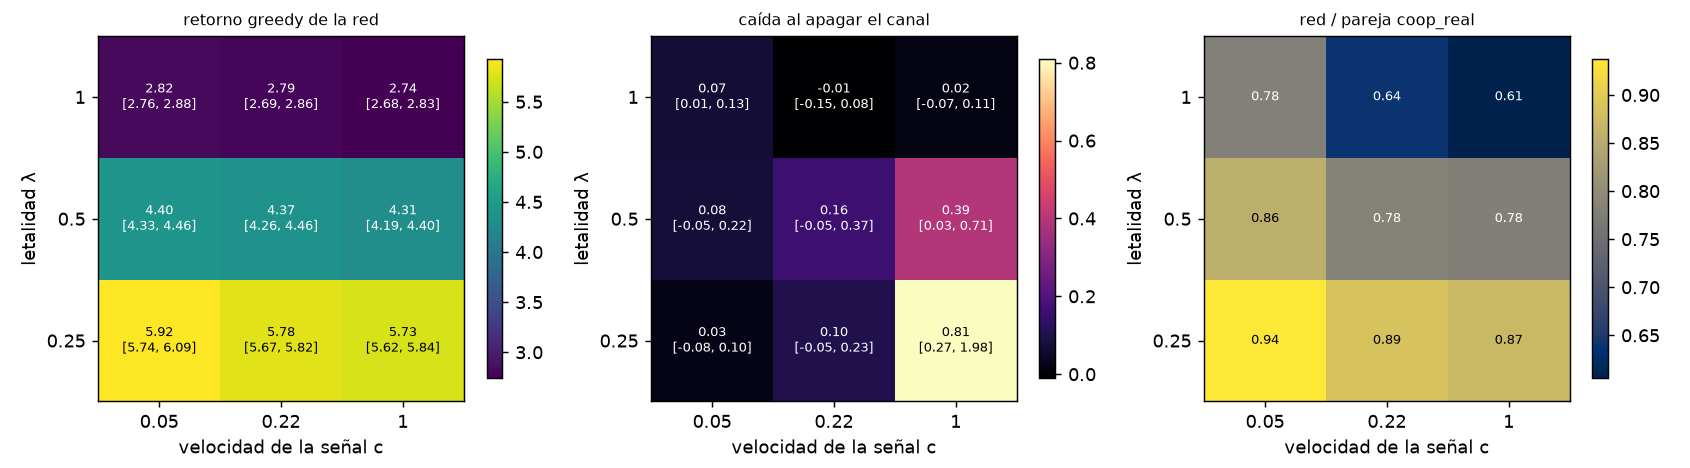
\includegraphics[width=0.92\textwidth]{barrido_entrenado.png}
\caption{Barrido $\lambda\times c$ con redes entrenadas (imitaci\'on y ajuste fino, 5 seeds por celda, 200 episodios, evaluaci\'on greedy). Afirmaci\'on visual: el retorno cae con la letalidad y casi no cambia con $c$. Los datos de origen est\'an en \codigo{analysis.barrido_entrenado}; la integridad cuantitativa de los ejes no se re-verific\'o para este documento.}
\label{fig:barrido}
\end{figure}

\begin{table}[H]
\centering\small
\begin{tabular}{@{}rrrrrrr@{}}
\toprule
$\lambda$ & $c$ & Red & Ca\'ida sin canal & \codigo{coop_real} & \codigo{solo} & Red / \codigo{coop_real} \\
\midrule
0.25 & 0.05 & $+5.92$ & $+0.03$ & $+6.74$ & $+5.97$ & 0.94 \\
0.25 & 0.22 & $+5.78$ & $+0.10$ & $+6.99$ & $+5.97$ & 0.89 \\
0.25 & 1.0 & $+5.73$ & $+0.81$ & $+6.99$ & $+5.97$ & 0.87 \\
0.5 & 0.05 & $+4.40$ & $+0.08$ & $+5.54$ & $+4.24$ & 0.86 \\
0.5 & 0.22 & $+4.37$ & $+0.16$ & $+5.99$ & $+4.24$ & 0.78 \\
0.5 & 1.0 & $+4.31$ & $+0.39$ & $+6.04$ & $+4.24$ & 0.78 \\
1.0 & 0.05 & $+2.82$ & $+0.07$ & $+3.97$ & $+2.85$ & 0.78 \\
1.0 & 0.22 & $+2.79$ & $-0.01$ & $+4.94$ & $+2.85$ & 0.64 \\
1.0 & 1.0 & $+2.74$ & $+0.02$ & $+5.02$ & $+2.85$ & 0.61 \\
\bottomrule
\end{tabular}
\caption{Barrido con redes entrenadas. Refugio caro (0.25), ruido 0.3, radio 0.45, 5 seeds, evaluaci\'on greedy. Las columnas de \codigo{coop_real} y \codigo{solo} salen de la matriz de cruce (200 episodios, 3 seeds de la red).}
\label{tab:barrido}
\end{table}

La dependencia del canal crece con la velocidad de la se\~nal a $\lambda=0.25$ y $0.5$, que es la forma que predice H2, pero son tres valores de $c$, una sola configuraci\'on de mundo y redes que parten de una imitaci\'on; por eso se describe como una tendencia y no como una frontera de fase. A $\lambda=1.0$ la red no usa el canal en ninguna celda. La red supera a \codigo{solo} solo con $\lambda=0.5$ (por $0.07$ a $0.16$); con $\lambda=0.25$ y $1.0$ queda entre $0.03$ y $0.24$ por debajo. En ninguna celda alcanza a \codigo{coop_real}.

\begin{figure}[H]
\centering
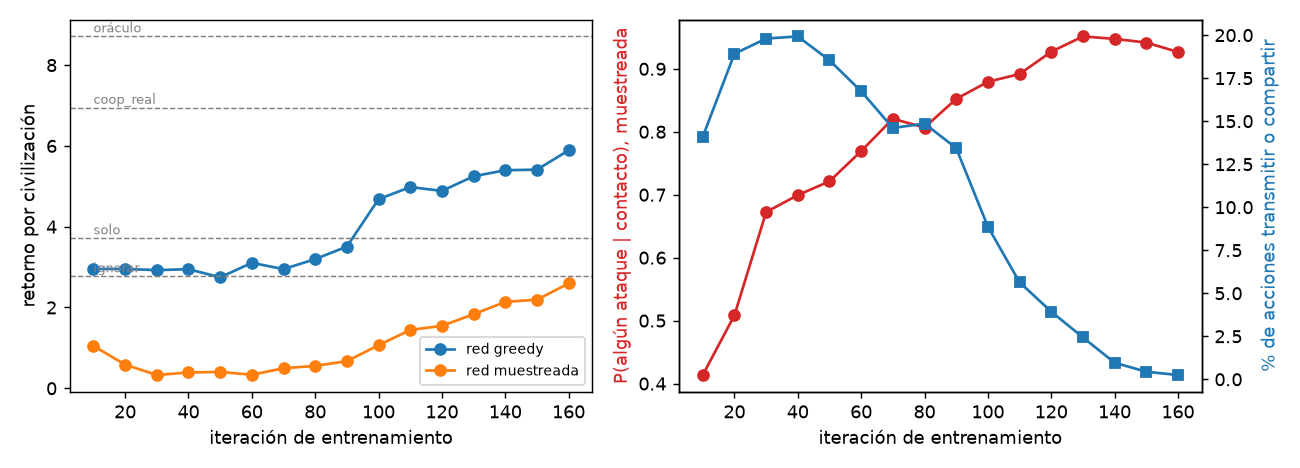
\includegraphics[width=0.85\textwidth]{evolucion_aprendizaje.png}
\caption{Evoluci\'on del aprendizaje de una seed a lo largo de 16 capturas del entrenamiento. Afirmaci\'on visual: al inicio 14\,\% a 20\,\% de las acciones son transmitir o compartir, pero apagar el canal no cambia nada (es exploraci\'on); con el entrenamiento cae a 0.2\,\%.}
\end{figure}

\subsection{Explotadores}

Cada explotador parte de su red principal y entrena 3.2 M pasos contra ella congelada. El explotador gana como mucho unos $0.2$ y la principal pierde entre $0.15$ y $0.26$; nadie dispara. Las redes no son fr\'agiles ante un adversario que se les ajusta, con un presupuesto de entrenamiento peque\~no.

\subsection{H3: enga\~no y se\~nales costosas}

\begin{table}[H]
\centering\small
\begin{tabular}{@{}lrr@{}}
\toprule
Fila contra columna & sin se\~nales costosas & con se\~nales costosas \\
\midrule
\codigo{coop_real} contra \codigo{coop_real} & $+6.00$ & $+5.75$ \\
\codigo{coop_real} contra \codigo{mentiroso} & $+3.97$ & $+3.82$ \\
\codigo{mentiroso} contra \codigo{coop_real} & $+6.00$ & $+6.00$ \\
\codigo{prudente} contra \codigo{prudente} & $+3.43$ & $+5.75$ \\
\codigo{prudente} contra \codigo{mentiroso} & $+3.43$ & $+3.27$ \\
\codigo{mentiroso} contra \codigo{prudente} & $+6.04$ & $+6.04$ \\
\codigo{solo} contra cualquiera & $+3.63$ & $+3.63$ \\
\bottomrule
\end{tabular}
\caption{Retornos con estrategias fijas, $\lambda=0.5$, $c=0.22$, refugio caro, ruido 0.3, 3 seeds, 200 episodios.}
\end{table}

Sin se\~nales costosas, el enga\~no paga: el mentiroso gana $+6.00$ contra \codigo{coop_real} y este $+3.97$. Con se\~nales costosas, \codigo{prudente} coopera consigo misma ($+5.75$) y no se contagia de las mentiras, pero no mejora a \codigo{coop_real} frente al mentiroso y el mentiroso sigue ganando: usa las mediciones verdaderas y devuelve falsas. Con este mecanismo H3 no se sostiene: verificar baja el retorno de cooperar en $0.25$ y no impide el aprovechamiento. Son estrategias fijas, sin redes entrenadas.

\subsection{H4: coaliciones}

Se entrenaron cinco seeds con 6 civilizaciones (3.2 M pasos, partiendo de la red clonada). Retorno greedy $+4.12$ [+3.96, +4.21], sin dependencia del canal. Con 12 episodios de $N=6$ por red, supervivencia entre 0.65 y 0.68, unos 17 mensajes por episodio, 1.2 comunidades y 100\,\% de los mensajes dentro de la comunidad: una sola comunidad que comparte con todas. La conclusi\'on depende del umbral de v\'inculo (con 3 mensajes una comunidad; con 6 se fragmenta; con 10 todas quedan aisladas), y sin un modelo nulo con la misma geometr\'ia no se puede atribuir la estructura que s\'i hay a algo distinto de la distancia y la velocidad de la se\~nal. Con estos datos H4 no se observa, y queda como pregunta abierta para el entorno.

\subsection{Estimar $N$ sin entrenar}

Evaluar una red con otro n\'umero de civilizaciones sin reentrenar (40 episodios, $\lambda=0.5$, $c=0.22$):

\begin{table}[H]
\centering\small
\begin{tabular}{@{}lrrrr@{}}
\toprule
Red & $N=2$ & $N=4$ & $N=6$ & $N=8$ \\
\midrule
Entrenada con 2 civilizaciones & $+4.22$ & $+3.32$ & $+2.52$ & $+2.59$ \\
Entrenada con 6 civilizaciones & $+4.17$ & $+4.40$ & $+4.22$ & $+4.10$ \\
\bottomrule
\end{tabular}
\caption{Retorno en greedy de dos redes por familia evaluadas con distinto $N$ sin reentrenar. Dos seeds por red; la densidad cambia con $N$, as\'i que los retornos entre tama\~nos no son del todo comparables.}
\end{table}

Las redes de 2 civilizaciones pierden cerca de 40\,\% a $N=6$; la de 6 queda entre $+4.1$ y $+4.4$ de 2 a 8. Para $N=4$ y 8 sirve la de 6 como estimaci\'on, y medir su error requerir\'a entrenar una red con ese tama\~no.

\subsection{Estado de las hip\'otesis}

\begin{table}[H]
\centering\small
\begin{tabular}{@{}l p{4cm} p{8cm}@{}}
\toprule
Hip. & Estado & Raz\'on \\
\midrule
H1 & Confirmada & Con $\lambda=0$ apagar el canal no cambia el retorno, con estrategias fijas y con redes (5 seeds) \\
H2 & Apoyada en parte & La dependencia del canal crece con $c$ a $\lambda$ bajo (tres valores de $c$, un mundo, redes con imitaci\'on); es una tendencia y no una frontera de fase \\
H3 & Pregunta abierta & Con estrategias fijas, verificar no impide el aprovechamiento y cuesta 0.25; falta medirla con redes entrenadas \\
H4 & Pregunta abierta & Se observa una sola comunidad que comparte con todas; el resultado depende del umbral de v\'inculo y requiere un modelo nulo \\
H5 & Pregunta abierta & No se observa bimodalidad entre seeds en el barrido; como la imitaci\'on reduce la varianza por construcci\'on, queda por probar sin ella \\
\bottomrule
\end{tabular}
\caption{Estado de las hip\'otesis al cierre de este documento.}
\end{table}

\subsection{Pruebas del c\'odigo}

El repositorio incluye pruebas automatizadas de los invariantes del entorno (recursos no negativos, muertos que no act\'uan, se\~nales que viajan a velocidad $c$) y de las estrategias fijas y la exportaci\'on. En la \'ultima ejecuci\'on de las pruebas de la demo pasaron 9 y fallaron 2 por un error de permisos de Windows sobre la carpeta temporal de \codigo{pytest}, ajeno a la l\'ogica probada. \codigo{ruff} no reporta errores.

%% ------------------------------------------------------------------
\section{Conclusi\'on}

El proyecto construy\'o un entorno donde comunicarse tiene valor funcional y costo de exposici\'on, y midi\'o ese valor con estrategias fijas antes de pedirles a las redes que lo descubrieran. Tres resultados sostienen la conclusi\'on:

\begin{enumerate}
\item Cooperar rinde cuando la anomal\'ia es costosa (hasta $+3.9$ de retorno en una celda con estrategias fijas) y no rinde cuando no lo es ($\lambda=0$). El canal no filtra informaci\'on.
\item El cuello de botella con agentes entrenados es el descubrimiento, no el valor de cooperar: desde cero las redes se quedan en $+2.84$, y con imitaci\'on llegan a $+4.37$ de un techo de $+5.99$.
\item H1 se confirma, H2 se apoya en parte, y H3, H4 y H5 quedan como preguntas abiertas para este entorno. Se reportan los resultados que no confirmaron la hip\'otesis con el mismo detalle que los que s\'i.
\end{enumerate}

\textbf{Alcance.} Los resultados corresponden a una sola familia de mundo para el barrido con redes, tres valores por eje, cinco seeds, redes que parten de una imitaci\'on, estrategias fijas en H3 y en la mayor parte de los diagn\'osticos, y una corrida de $N=6$ con 12 episodios por red. Describen este entorno y estas reglas; no son una afirmaci\'on sobre civilizaciones reales ni sobre la teor\'ia del bosque oscuro.

\textbf{Siguientes pasos.} El proyecto se puede extender entrenando con $N$ grande y con se\~nales costosas, a\~nadiendo un modelo nulo para las comunidades, un barrido con m\'as valores de $c$, y repitiendo la imitaci\'on con otros expertos.

\textbf{Repositorio.} El c\'odigo y este documento est\'an en el repositorio p\'ublico \url{https://github.com/SergioAle210/RL-DarkForest}. Los comandos para reproducir cada cifra est\'an en \codigo{docs/DIAGNOSTICO_DISENO.md} y la demo se lanza con \codigo{uv run python -m demo.servidor}.

%% ------------------------------------------------------------------
\begin{thebibliography}{99}
\small
\bibitem{liu2015} Liu, C. (2015). \textit{The Dark Forest} (J. Martinsen, trad.). Tor Books. (Obra original, 2008.)
\bibitem{hansen2004} Hansen, E. A., Bernstein, D. S. y Zilberstein, S. (2004). Dynamic programming for partially observable stochastic games. \textit{Proceedings of the 19th AAAI Conference on Artificial Intelligence}.
\bibitem{schulman2017} Schulman, J., Wolski, F., Dhariwal, P., Radford, A. y Klimov, O. (2017). Proximal policy optimization algorithms. arXiv:1707.06347.
\bibitem{dewitt2020} de Witt, C. S., Gupta, T., Makoviichuk, D., Makoviychuk, V., Torr, P. H. S., Sun, M. y Whiteson, S. (2020). Is independent learning all you need in the StarCraft multi-agent challenge? arXiv:2011.09533.
\bibitem{yu2022} Yu, C., Velu, A., Vinitsky, E., Gao, J., Wang, Y., Bayen, A. y Wu, Y. (2022). The surprising effectiveness of PPO in cooperative multi-agent games. \textit{Advances in Neural Information Processing Systems}, 35. arXiv:2103.01955.
\bibitem{cho2014} Cho, K., van Merri\"enboer, B., Gulcehre, C., Bahdanau, D., Bougares, F., Schwenk, H. y Bengio, Y. (2014). Learning phrase representations using RNN encoder-decoder for statistical machine translation. \textit{EMNLP 2014}. arXiv:1406.1078.
\bibitem{heinrich2016} Heinrich, J. y Silver, D. (2016). Deep reinforcement learning from self-play in imperfect-information games. arXiv:1603.01121.
\bibitem{ross2011} Ross, S., Gordon, G. J. y Bagnell, J. A. (2011). A reduction of imitation learning and structured prediction to no-regret online learning. \textit{Proceedings of the 14th International Conference on Artificial Intelligence and Statistics (AISTATS)}, PMLR 15, 627--635.
\bibitem{bradbury2018} Bradbury, J., Frostig, R., Hawkins, P., Johnson, M. J., Leary, C., Maclaurin, D., Necula, G., Paszke, A., VanderPlas, J., Wanderman-Milne, S. y Zhang, Q. (2018). JAX: composable transformations of Python+NumPy programs. \url{https://github.com/jax-ml/jax}.
\bibitem{rutherford2023} Rutherford, A. et al. (2023). JaxMARL: Multi-agent RL environments in JAX. arXiv:2311.10090.
\bibitem{taylor1978} Taylor, P. D. y Jonker, L. B. (1978). Evolutionary stable strategies and game dynamics. \textit{Mathematical Biosciences}, 40(1--2), 145--156.
\bibitem{crawford1982} Crawford, V. P. y Sobel, J. (1982). Strategic information transmission. \textit{Econometrica}, 50(6), 1431--1451.
\bibitem{spence1973} Spence, M. (1973). Job market signaling. \textit{The Quarterly Journal of Economics}, 87(3), 355--374.
\bibitem{foerster2016} Foerster, J. N., Assael, Y. M., de Freitas, N. y Whiteson, S. (2016). Learning to communicate with deep multi-agent reinforcement learning. \textit{Advances in Neural Information Processing Systems}, 29. arXiv:1605.06676.
\bibitem{lazaridou2020} Lazaridou, A. y Baroni, M. (2020). Emergent multi-agent communication in the deep learning era. arXiv:2006.02419.
\bibitem{kardashev1964} Kardashev, N. S. (1964). Transmission of information by extraterrestrial civilizations. \textit{Soviet Astronomy}, 8(2), 217--221.
\bibitem{sullivan2019} Sullivan, C. B. y Kaszynski, A. (2019). PyVista: 3D plotting and mesh analysis through a streamlined interface for the Visualization Toolkit (VTK). \textit{Journal of Open Source Software}, 4(37), 1450.
\bibitem{anthropicclaudecode} Anthropic. (2026). Claude Code: documentaci\'on. \url{https://code.claude.com/docs}.
\bibitem{agentskills} Agent Skills. (s.\,f.). Especificaci\'on del formato. \url{https://agentskills.io/specification}.
\end{thebibliography}

\end{document}
